\section{Appendix of Chapter 6}

\subsection{Proofs related to Augmented Gromov-Wasserstein} \label{appendix:agw}

\begin{proof}[Proof of \Cref{prop:basic_prop}]
  The proof of this proposition can be adapted directly from \citep{Vayer19b}.
  For self-contained purpose, we reproduce the proof here. Denote
  \begin{itemize}
      \item[$\bullet$] $(P_{\alpha}, Q_{\alpha})$ the optimal sample and feature couplings for
      $\agw_{\alpha}(\cX, \cY)$.

      \item[$\bullet$] $(P_0, Q_0)$ the optimal sample and feature couplings for
      $\coot(\cX, \cY)$ (corresponding to $\alpha = 0$).

      \item[$\bullet$] $P_1$ the optimal sample coupling for $\gw(\cX, \cY)$
      (corresponding to $\alpha = 1$).
  \end{itemize}
  Due to the suboptimality of $P_{\alpha}$ for GW and $(P_1, Q_0)$ for AGW, we have
  \begin{align}
      \alpha \langle L(C^X, C^Y) \otimes P_1, P_1 \rangle
      &\leq \alpha \langle L(C^X, C^Y) \otimes P_{\alpha}, P_{\alpha} \rangle
      + (1 - \alpha) \langle L(X, Y) \otimes Q_{\alpha}, P_{\alpha} \rangle \\
      &\leq \alpha \langle L(C^X, C^Y) \otimes P_1, P_1 \rangle
      + (1 - \alpha) \langle L(X, Y) \otimes Q_0, P_1 \rangle,
  \end{align}
  or equivalently
  \begin{align}
      \alpha \gw(\cX, \cY) \leq \agw_{\alpha}(\cX, \cY) \leq \alpha \gw(\cX, \cY)
      + (1 - \alpha) \langle L(X, Y) \otimes Q_0, P_1 \rangle.
  \end{align}
  Similarly, we have
  \begin{align}
      (1 - \alpha) \coot(\cX, \cY) &\leq \agw_{\alpha}(\cX, \cY) \\
      &\leq (1 - \alpha) \coot(\cX, \cY) + \alpha \langle L(C^X, C^Y) \otimes P_0, P_0 \rangle.
  \end{align}
  The interpolation property then follows by the sandwich theorem.
\end{proof}

We thank professor Facundo Memoli for pointing out the proof techniques,
which allow to establish the metric properties of AGW.
Let us first state the following lemma.
\begin{lemma}
    \label{lemma:triangle_ineq}
    Let $d_X: X^2 \to \bbR^+$ and $d_Y: Y^2 \to \bbR^+$ be two functions.
    For any $p \geq 1$ and $\alpha, \beta \geq 0$, define the function
    $d: (X \times Y)^2 \to \bbR^+$ by $d((x_1, y_1), (x_2, y_2)) = \big[ \alpha d^p_X(x_1, x_2) + \beta d^p_Y(y_1, y_2) \big]^{1/p}$.
    If $d_X$ and $d_Y$ satisfy the triangle inequality, then so does $d$.
\end{lemma}
\begin{proof}[Proof of \Cref{lemma:triangle_ineq}]
    WLOG, assume $\alpha = \beta = 1$ (otherwise consider
    $\widehat{d}_X = \alpha^{1/p} d_X$ and $\widehat{d}_Y = \beta^{1/p} d_Y$).
    For convenience, denote $z = (x, y)$. We have
    \begin{align}
        d^p(z_1, z_2) &= d^p_X(x_1, x_2) + d^p_Y(y_1, y_2) \\
        &\leq \Big[ d_X(x_1, x_3) + d_X(x_3, x_2) \Big]^p
        + \Big[d_Y(y_1, y_3) + d_Y(y_3, y_2) \Big]^p \\
        &\leq \Big[ (d^p_X(x_1, x_3) + d^p_Y(y_1, y_3))^{1 / p}
        + (d^p_X(x_3, x_2) + d_Y^p(y_3, y_2))^{1/p} \Big]^p \\
        &=\Big[ d(z_1, z_3) + d(z_3, z_2) \Big]^p,
    \end{align}
    where the second inequality is due to the Minkowski's inequality in case of counting measure:
    $\big[ (a + b)^p + (c+d)^p \big]^{1/p} \leq (a^p + c^p)^{1 / p} + (b^p + d^p)^{1/p}$,
    for any $a,b,c,d \geq 0$ and $p \geq 1$. The result then follows.
\end{proof}

\begin{proof}[Proof of \Cref{prop:metric_agw}]
    Recall that in GW, Wasserstein, COOT distances, there are only two crucial
    components in the proof of the triangle inequality: the glueing lemma
    and the fact that the objectives functions satisfy the triangle inequality.
    More precisely,
      \begin{itemize}
          \item[$\bullet$] In Wasserstein distance: $W_p(\cX, \cY)= \inf_{\pi \in U(\mu_x, \mu_y)} ||d||_{L^p(\mu)}$, where $d: X \times Y \to \bbR^+$ is
          a distance function. Here $d(x, y) \leq d(x, z) + d(y, z)$.
          \item[$\bullet$] In GW distance: $\gw_p(\cX, \cY)= \inf_{\pi \in U(\mu_x, \mu_y)} ||\Gamma_{XY}||_{L^p(\mu \otimes \mu)}$,
          where $\Gamma_{XY} : (X \times Y)^2 \to \bbR^+$ defined by
          $\Gamma_{XY}((x, y), (x', y')) := |d_X(x, x') - d_Y(y, y')|$. Here,
          $\Gamma_{XY}((x, y), (x', y')) \leq \Gamma_{YZ}((y, z), (y', z')) + \Gamma_{XZ}((x, z), (x', z'))$.
      \end{itemize}
      For this reason, in order to establish the triangle inequality for AGW,
      it is enough to show that its objective function
      satisfies the triangle inequality. Note that,
      \begin{align}
          &L_{\agw}(\cX, \cY) \\
          &= \alpha \sum_{i,j,k,l} |C^X_{i,j} - C^Y_{k,l}|^p P_{i,k} P_{j, l}
          + (1 - \alpha) \sum_{i,j,k,l} |X_{i,j} - Y_{k,l}|^p P_{i,k} Q_{j,l} \\
          &= \sum_{i,j,k,l,m,n} \Big[ \alpha |C^X_{i,j} - C^Y_{k,l}|^p
          + (1 - \alpha) |X_{i,m} - Y_{k,n}|^p \Big] P_{i,k} P_{j, l} Q_{m,n} \\
          &= \iiint \Big[ \alpha |C^X(x, x') - C^Y(y, y')|^p
          + (1 - \alpha) |x_{m} - y_{n}|^2 \Big] \mathrm{d}P(x, y) \; \mathrm{d}P(x', y') \; \mathrm{d}Q(x_m, y_n) \\
          &= || F_{XY} ||^p_{L^p(P \otimes P \otimes Q)},
      \end{align}
      where $F_{XY}: (\widetilde{X} \times \widetilde{Y} \times \bbR)^2 \to \bbR^+$ is defined by
      \begin{align}
          F_{XY}((x, x', x_m), (y, y', y_n)) :=
          \Big( \alpha |C^X(x, x') - C^Y(y, y')|^p + (1 - \alpha) |x_{m} - y_{n}|^p \Big)^{1/p}.
      \end{align}
      Here, the sets $\widetilde{X}, \widetilde{Y}$ contain $n_x, n_y$ rows of matrices $X, Y$, respectively.
      The scalars $x_m, y_n$ represent the $m^{\text{th}}, n^{\text{th}}$ coordinates of
      the vectors $x \in \widetilde{X}, y \in \widetilde{Y}$, respectively.
      By \Cref{lemma:triangle_ineq}, since $\Gamma_{XY}: ((x,y), (x',y')) \to |C^X(x, x') - C^Y(y, y')|$
      and $|\cdot|: (a, b) \to |a-b|$ satisfy the triangle inequality,
      so does $F_{XY}$. Now, the proof of the triangle inequality of AGW can be
      adapted immediately from that of any distance amongst Wasserstein, GW and COOT.

      Fixing $\alpha \in [0,1)$, suppose that there exist two bijections
      $\sigma_r \in \mathbb S_{n_x}$ and $\sigma_c \in \mathbb S_{d_x}$ such that
      $X_{ij} = Y_{\sigma_r(i), \sigma_c(j)}$. Denote $P, Q$ the permutation matrices
      corresponding to the permutation $\sigma_r, \sigma_c$, respectively.
      Then, for any $q \geq 0$,
      \begin{align}
        (C^X_{i,j})^q &= \sum_{d = 1}^{d_x} |X_{id} - X_{jd}|^q
        = \sum_{d = 1}^{d_x} |Y_{\sigma_r(i), \sigma_c(d)} - Y_{\sigma_r(j), \sigma_c(d)}|^q \\
        &= \sum_{d' = 1}^{d_y} |Y_{\sigma_r(i), d'} - Y_{\sigma_r(j), d'}|^q
        = (C^Y_{\sigma_r(i), \sigma_r(j)})^q,
      \end{align}
      where recall that, we must have $d_x = d_y$. We deduce that
      \begin{align}
        \sum_{i,j,k,l} |C^X_{i,j} - C^Y_{k,l}|^p P_{ik} P_{jl} =
        \sum_{i,j} |C^X_{i,j} - C^Y_{\sigma_r(i), \sigma_r(j)}|^p = 0.
      \end{align}
      Clearly, $\sum_{i,j,k,l} |X_{i,j} - Y_{k,l}|^p P_{ik} Q_{jl} = 0$.
      So, $\agw_{\alpha}(\cX, \cY) = 0$. Conversely,
      if $\agw_{\alpha}(\cX, \cY) = 0$, then we must have $\coot(\cX, \cY) = 0$.
      By Proposition 3.1 in \citep{Redko20}, there exist two bijections
      $\sigma_r \in \mathbb S_{n_x}$ and $\sigma_c \in \mathbb S_{d_x}$ such that
      $X_{ij} = Y_{\sigma_r(i), \sigma_c(j)}$.
\end{proof}

\paragraph{Remark.} The above proof of the triangle inequality of AGW can be
adapted immediately to the fused GW \citep{Vayer19b}. In particular, FGW
defines a proper metric, rather than just a semi-metric as stated in Theorem 6.3
in \citep{Vayer19b}.

%%%%%%%%%%%%%%%%%%%%%%%%%%%%%%%%%%%%%%
\begin{proof}[Proof of \Cref{corr:hermitian}]
  This proof is based on the personal communication with professor Will Sawin
  on his discussion on \url{https://mathoverflow.net/questions/420319/why-is-the-set-of-hermitian-matrices-with-repeated-eigenvalue-of-measure-zero}.
  We thank him for his invaluable support during the submission of our paper.

  First, let us recall the Schwartz-Zippel lemma. Denote $F(x_1, ..., x_n)$ a multivariate polynomial.
  Its total degree is the maximum of the sums of the powers of the variables in any monomial.
  The Schwartz-Zippel lemma states that: let $F(x_1, ..., x_n)$ be a nonzero multivariate polynomial
  of total degree $d$ and $S$ be a finite subset of $\bbR$. Denote
  $Z_S := \{ (x_1, ..., x_n) \in S^n : F(x_1, ..., x_n) = 0 \}$ the set of zeros of $F$ on $S^n$.
  Then $| Z_S | \leq d |S|^{n-1}$.

  Note that, the set of Hermitian matrices of size $n$ forms a finite-dimensional real vector space.
  In particular, it is isomorphic to the Euclidean space $\bbR^{n^2}$.
  Denote $I$ set of Hermitian matrices of size $n$ with repeated eigenvalues.
  It is enough to show that $I$ has measure zero. We have $I \simeq E$,
  for some $E \subset \bbR^{n^2}$. By Proposition 4 in \citep{Stein05},
  since $I$ is closed (see page 56 in \citep{Tao12}), it is measurable.
  If $I$ does not have zero measure,
  then the intersection $E \cap [0, 1]^{n^2}$ has positive measure $p > 0$. If,
  for each $i \in [n^2]$, we sample $m$ i.i.d coordinates uniformly in $[0, 1]$,
  then we have $m^{n^2}$ points uniformly distributed in $[0, 1]^{n^2}$. So,
  the expected number of points lying in $E$ is $pm^{n^2}$.

  On the other hand, recall that a (Hermitian) matrix has repeated eigenvalues if and only if
  the discriminant of its characteristic polynomial is zero. Moreover,
  the discriminant of the characteristic polynomial is a polynomial in $n^2$ entries of the matrix.
  Thus, the measure of $I$ (or, equivalently $E$) is the measure of the set of values of these
  $n^2$ variables which make a certain polynomial of total degree $d$ vanish.
  By Schwartz-Zippel lemma, on average, there are at most $d m^{n^2-1}$ points in $E$.
  By choosing $m > d / p$, we obtain a contradiction. Thus $E$ (or equivalently $I$)
  must have zero measure.
\end{proof}

%%%%%%%%%%%%%%%%%%%%%%%%%%%%%%%%%%%%%%%%%%%%%%
\begin{proof}[Proof of \Cref{thm:invariant}]
  For $0 < \alpha < 1$, if $\agw_{\alpha}(\cX, \cY) = 0$, then
  $\gw(\cX, \cY) = \coot(\cX, \cY) = 0$. In particular,
  $X$ and $Y$ must have the same shape, so $X, Y \in \bbR^{n \times d}$.
  As $\gw(\cX, \cY) = 0$, there exists an isometry from $X$ to $Y$. Note that every isometry from
  $\bbR^d$ to $\bbR^d$ is a composition of at most $d+1$ reflections
  (see, for example, Corollary A.7 in \citep{Konrad}). So, $Y = X O$, for some $O \in \cO_d$.
  As $\coot(\cX, \cY) = 0$, there exist two permutation matrices $P \in \cP_n, Q_1 \in \cP_d$ such that $Y = P X Q_1$.
  We deduce that $X O = P X Q_1$, or equivalently $X = P X Q$, for
  $Q = Q_1 O^T \in \cO_d$. We will show that $Q$ is symmetric.

  Indeed, consider the singular value decomposition of $X$, \ie,
  $X = U \Sigma V^T$, where $U \in \bbR^{n \times d}$ such that $U^T U = I_d$,
  $V \in \cO_d$ and $\Sigma \in \bbR^{d \times d}$ is a diagonal matrix
  whose diagonal contains $d$ strictly decreasing singular values (since $n \geq d$). As $X = P X Q$,
  we have $U \Sigma V^T = (PU) \Sigma (V^T Q)$. For $i \in [d]$, let $u_i \in \bbR^n$
  and $v_i \in \bbR^d$ be columns of $U$ and $V$, respectively.
  As the singular values are positive and distinct, the columns are unique up to
  the sign change of both columns in $U$ and $V$. This means $u_i = \pm Pu_i$ and
  $v_i = \pm Q^T v_i$. In other words, $\pm 1$ are eigenvalues of $P$ and $Q^T$, and
  $u_i, v_i$ are their corresponding eigenvectors, respectively. Denote $D \in \bbR^{d \times d}$
  any diagonal matrix whose diagonal values are in $\{ \pm 1 \}$, then
  $Q^T = V D V^{-1} = V D V^T = Q$. So, $Q$ is symmetric.
  \Cref{thm:invariant} then follows by observing that $O = Q^T Q_1$.
\end{proof}

%%%%%%%%%%%%%%%%%%%%%%%%%%%%%%%%%%%%%%%%%%%%%%%%%%
\begin{lemma}
\label{prop:coot_invariant}
    For $p=2$, COOT is weakly invariant to translation.
\end{lemma}
\begin{proof}[Proof of \Cref{prop:coot_invariant}]
For any $P \in U(\mu_1^X, \mu_1^Y), Q \in U(\mu_2^X, \mu_2^Y)$ and $c \in \bbR$, we have
\begin{align}
    \sum_{i,j,k,l} (X_{ik} - Y_{jl} - c)^2 P_{ij} Q_{kl}
    &= \sum_{i,j,k,l} (X_{ik} - Y_{jl})^2 P_{ij} Q_{kl}
    - 2c \sum_{i,j,k,l} (X_{ik} - Y_{jl}) P_{ij} Q_{kl} + c^2.
\end{align}
Now,
\begin{align}
    \sum_{i,j,k,l} (X_{ik} - Y_{jl}) P_{ij} Q_{kl}
    &= \sum_{i,j,k,l} X_{ik} P_{ij} Q_{kl} - \sum_{ijkl} Y_{jl} P_{ij} Q_{kl} \\
    &= \sum_{i,k} X_{ik} \left( \sum_j P_{ij} \right) \left( \sum_l Q_{kl} \right)
    - \sum_{j,l} Y_{jl} \left( \sum_i P_{ij} \right) \left( \sum_k Q_{kl} \right) \\
    &= \sum_{i,k} X_{ik} (\mu_1^X)_i (\mu_2^X)_j \mu'_k - \sum_{j,l} Y_{jl} (\mu_1^Y)_j (\mu_2^Y)_l \\
    &= (\mu_1^X)^T X \mu_2^X - (\mu_1^Y)^T Y \mu_2^Y.
\end{align}
So, $\coot(\cX, \cY + c) = \coot(\cX, \cY) -
2 c \left( (\mu_1^X)^T X \mu_2^X - (\mu_1^Y)^T Y \mu_2^Y \right) + c^2$.
This implies that COOT is weakly invariant to translation.
\end{proof}

\begin{proof}[Proof of \Cref{prop:invariant}]
Note that the GW term in AGW remains unchanged by translation.
By adapting the proof of \Cref{prop:coot_invariant}, for $p=2$, we obtain
\begin{align}
    \agw_{\alpha}(\cX, \cY + c) = \agw_{\alpha}(\cX, \cY) + (1 - \alpha) \left[ c^2
    - 2 c \left( (\mu_1^X)^T X \mu_2^X - (\mu_1^Y)^T Y \mu_2^Y \right) \right].
\end{align}
The result then follows.
\end{proof}

%%%%%%%%%%%%%%%%%%%%%%%%%%%%%%
\subsection{Experimental Set-up Details} \label{subsec:appendix_expe_agw}

\subsubsection{MNIST Illustrations} We align $1000$ images of hand-written digits from
the MNIST dataset with $1000$ images from the USPS dataset. Each dataset is subsampled to
contain $100$ instances of each of the $10$ possible digits ($0$ through $9$),
using the random seed of $1976$. We set all marginal distributions to uniform,
and use cosine distances for GW and AGW. We consider both the entropically regularized and
non-regularized versions for all methods. For entropic regularization, we sweep a grid of
$\varepsilon_1, \varepsilon_2 (\textrm{ =if applicable}) \in [5e-4, 1e-3, 5e-3, 1e-2, 5e-2, 1e-1, 5e-1]$.
For AGW, we consider $[0.1, 0.2, 0.3, ..., 0.9]$, and present results with the best-performing
hyperparameter combination of each method, as measured by the percent accuracy of matching images
from the same digit across the two datasets.

\subsubsection{Single-cell multi-omic alignment experiments}

% As a real-world application of AGW, we align single-cell data from different measurement domains.
% Optimal transport has recently been applied to this problem in computational biology by
% multiple groups \citep{Demetci20, Pamona, UniPort}. To briefly introduce the problem:
% Biologists are interested in jointly studying multiple genomic (\ie, ``multi-omic'')
% aspects of cells to determine biologically relevant patterns in their co-variation.
% Such studies reveal how the different molecular aspects of a cell's genome (\eg,
% its 3D structure, chemical modifications it undergoes, activity levels of its genes, etc)
% interact to regulate the cell's response to its environment. These studies are of interest
% for both fundamental biology research, as well as drug discovery applications.
% However, as \citep{liu_et_al:LIPIcs:2019:11040} describe, combining multiple measurements on the
% same cells is experimentally difficult. Consequently, computational approaches are developed
% to integrate data from different measurement modalities using biologically relevant cell populations.
% In this paper, we apply AGW to jointly align both cells and genomic features of single-cell datasets.
% This is a novel direction in the application of optimal transport (OT) to
% single-cell multi-omic alignment tasks, as the existing OT-based algorithms only align cells.

\paragraph{Datasets} We largely follow the first paper that applied OT to
single-cell multi-omic alignment task \citep{Demetci20} in our experimental set-up and
use four simulated datasets and three real-world single-cell multi-omic datasets to benchmark
our cell alignment performance.

Three of the simulated datasets have been generated by
\citep{liu_et_al:LIPIcs:2019:11040} by non-linearly projecting 600 samples from a common
2-dimensional space onto different 1000- and 2000-dimensional spaces with 300 samples in each.
% In the first simulation, the data points in each domain form a bifurcating tree structure
% that is commonly seen in cell populations undergoing differentiation. The second simulation
% forms a three-dimensional Swiss roll. Lastly, the third simulation forms a circular frustum
% that resembles what is commonly observed when investigating the cell cycle.
% These datasets have been previously used for benchmarking by other cell-cell alignment methods
% \citep{liu_et_al:LIPIcs:2019:11040,singh20,cao2020unsupervised, Pamona,Demetci20}.
% We refer to these datasets as ``Sim 1'', ``Sim 2'', and ``Sim 3'', respectively.

We include a fourth simulated dataset generated by \citep{Demetci20} using a single-cell RNA-seq
data simulation package in R, called Splatter \citep{zappia2017splatter}.
We refer to this dataset as ``Synthetic RNA-seq''. This dataset includes a simulated gene expression
domain with 50 genes and 5000 cells divided across three cell types and another domain created
by non-linearly projecting these cells onto a 500-dimensional space. As a result of
their generation schemes, all simulated datasets have ground-truth 1-1 cell
correspondence information. We use this information solely for benchmarking.
We do not have access to ground-truth feature relationships in these datasets,
so we exclude them from feature alignment experiments.

Additionally, we include three real-world single-cell sequencing datasets in our experiments.
To have ground-truth information on cell correspondences for evaluation, we choose
three co-assay datasets which have paired measurements on the same individual cells:
an scGEM dataset \citep{cheow2016}, a SNARE-seq dataset \citep{SNAREseq}, and
a CITE-seq dataset \citep{CITEseq} (these are exceptions to the experimental challenge
described above). These first two datasets have been used by existing
OT-based single-cell alignment methods
\citep{cao2020unsupervised, singh20, Demetci20, Pamona, Demetci22},
while the last one was included in the evaluations of a non-OT-based alignment method,
bindSC \citep{bindSC}.

In addition to these three datasets,
we include a fourth single-cell dataset, which contains data from the same measurement modality
(\ie, gene expression) but from two different species: mouse \citep{mouse} and
bearded lizard \citep{lizard}. Our motivation behind including this dataset is
to demonstrate the effects of both sample-level (\ie, cell-level) and
feature-level (\ie, gene-level) supervision on alignment qualities.
We refer to this dataset as the ``cross-species dataset'', which contains 4,187 cells
from lizard pallium (a brain region) and 6,296 cells from the mouse prefrontal cortex.
The two species share a subset of their features: 10,816 paralogous genes.
Each also has species-specific genes: 10,184 in the mouse dataset and 1,563 in the lizard dataset.
% The data comes from different species, so there is no 1--1 correspondence between cells.
% However, the two species contain cells from similar cell types.
% Unlike the other single-cell dataset, there is a subset of the features (the paralogous genes)
% that have 1--1 correspondences across the two domains (domains are defined by species in this dataset).

\paragraph{Baselines and hyperparameter tuning}
We benchmark AGW's performance on single-cell alignment tasks against three algorithms:
(1) COOT \citep{Redko20}, (2) SCOT \citep{Demetci20}, which is a Gromov-Wasserstein OT-based
algorithm that uses k-nearest neighbor (kNN) graph distances on dimensionality reduced datasets
(top 30 principal components for gene expression domains and simulated domains,
15-25 topics with latent dirichlet allocation for other measurement domains)
as intra-domain distance matrices. This choice of distances has been shown to perform
better than Euclidean distances, cosine distances by \citep{Demetci20}, and bindSC \citep{bindSC}.
For consistency, we keep the intra-domain distance computations the same for AGW and UGW, too.
Among all baselines, bindSC is not an OT-based algorithm: It employs bi-order canonical correlation
analysis to perform alignment. We include it as a benchmark as it is the only existing
single-cell alignment algorithm that can perform feature alignments (in addition to cell alignments)
for a few limited types of measurement modalities.

When methods share similar hyperparameters in their formulation (\eg,
entropic regularization constant, $\varepsilon$ for methods that employ OT),
we use the same hyperparameter grid to perform their tuning. Otherwise,
we refer to the publication and the code repository for each method to choose a hyperparameter range.
For SCOT, we tune four hyperparameters: $k \in \{20, 30, \dots, 150\}$, the number of neighbors
in the cell neighborhood graphs, $\varepsilon \in \{5e-4, 3e-4, 1e-4, 7e-3, 5e-3, \dots, 1e-2 \}$,
the entropic regularization coefficient for the optimal transport formulation. Similarly,
for both COOT and AGW, we sweep
$\varepsilon_1, \varepsilon_2 \in \{5e-4, 3e-4, 1e-4, 7e-3, 5e-3, \dots, 1e-2 \}$
for the coefficients of entropic regularization over the sample and feature alignments.
We use the same intra-domain distance matrices in AGW as in SCOT (based on kNN graphs).
For all OT-based methods, we perform barycentric projection to complete the alignment.

For bindSC, we choose the coupling coefficient that assigns weight to the
initial gene activity matrix $\alpha \in \{0, 0.1, 0.2, \dots 0.9\}$ and
the coupling coefficient that assigns a weight factor to multi-objective function
$\lambda \in \{0.1, 0.2, \dots, 0.9\}$. Additionally, we choose the number of canonical vectors
for the embedding space $K \in \{3, 4, 5, 10, 30, 32\}$.  For all methods,
we report results with the best-performing hyperparameter combinations.

\paragraph{Evaluation Metrics} When evaluating cell alignments, we use a metric previously used
by other single-cell multi-omic integration tools
\citep{liu_et_al:LIPIcs:2019:11040,singh20,cao2020unsupervised,Demetci20,Pamona,Demetci22,bindSC}
called ``fraction of samples closer than the true match'' (FOSCTTM). For this metric,
we compute the Euclidean distances between a fixed sample point and all the data points
in the other domain. Then, we use these distances to compute the fraction of samples
that are closer to the fixed sample than its true match and then average these values
for all the samples in both domains. This metric measures alignment error, so the lower values
correspond to higher-quality alignments.

We investigate the accuracy of feature correspondences recovered to assess feature alignment
performance. We mainly use two real-world datasets for this task - CITE-seq,
and the cross-species scRNA-seq datasets (results on SNARE-seq and scGEM datasets
are qualitatively evaluated due to the lack of ground-truth information). For the CITE-seq dataset,
we expect the feature correspondences to recover the relationship between the 25 antibodies
and the genes that encode them. To investigate this, we simultaneously align the cells and
features of the two modalities using the 25 antibodies and 25 genes in an unsupervised manner.
We compute the percentage of 25 antibodies whose strongest correspondence is their encoding gene.

For the cross-species RNA-seq dataset, we expect alignments between (1) the cell-type annotations
common to the mouse and lizard datasets, namely excitatory neurons, inhibitory neurons,
microglia, OPC (Oligodendrocyte precursor cells), oligodendrocytes, and endothelial cells
and (2) between the paralogous genes. For this dataset, we generate cell-label matches
by averaging the rows and columns of the cell-cell alignment matrix yielded by AGW based on
these cell annotation labels. We compute the percentage of these six cell-type groups that
match as their strongest correspondence. For feature alignments, we compute the percentage
of the 10,816 shared genes that are assigned to their corresponding paralogous gene with
their highest alignment probability. For this dataset, we consider providing supervision at
increasing levels on both sample and feature alignments. For feature-level supervision,
$20\%$ supervision means setting the alignment cost of $\sim 20\%$ of the genes with
their paralogous pairs to $0$. For sample-level supervision, $20\%$ supervision corresponds
to downscaling the alignment cost of $\sim 20\%$ of the mouse cells from the aforementioned
seven cell types with the $\sim 20\%$ of lizard cells from their corresponding cell-type by
$\frac{1}{\textrm{\# lizard cells in the same cell-type}}$.

% \subsubsection{Heterogeneous domain adaptation experiments}
% We evaluate AGW against GW and COOT on source-target pairs from the Caltech-Office dataset
% \citep{Saenko10}by considering all pairs between the three domains: Amazon (A), Caltech-$256$ (C),
% and Webcam (W), similarly to Redko \textit{et al}. We randomly choose 20 samples per class
% and perform adaptation from CaffeNet to GoogleNet and repeat it 10 times.
% We report the average performance of each method along with the standard deviation.
% Differently than Redko \textit{et al.}, we (1) unit normalize the dataset prior to alignment
% as we empirically found it to boost all methods' average performance compared to using
% unnormalized datasets, (2) use cosine distances when defining intra-domain distance matrices
% for GW and AGW, as we found them to perform better than Euclidean distances,
% and (3) report results after hyperparameter tuning methods for each pair of datasets.
% Specifically, for each pair of (A)-(C), (A)-(W), etc, we sweep a hyperparameter grid over
% 5 runs of random sampling, choose the best-performing combination, and run
% 10 runs of random sampling to report results. For all methods that allow for entropic regularization,
% we consider their version with no entropic regularization (either on the sample-level alignments,
% feature-level alignments, or both), along with various levels of regularization.
% For entropic regularization over sample alignments, we consider
% $\varepsilon_1 \in [ 5e-4, 1e-3, 5e-3, 1e-2, 5e-2, 0.1] $.  For entropic regularization over
% feature alignments in COOT and AGW, we consider $\varepsilon_2 \in [ 5e-4, 1e-3, 5e-3, 1e-2, 5e-2, 0.1]$.
% As the interpolation coefficient of AGW, we consider $\alpha \in [ 0.1, 0.2, ..., 0.9]$.

%%%%%%%%%%%%%%%%%%%%%%%%%%%%%%
% \subsection{Empirical Runtime Analysis} \label{subsec:chap5_runtime}

% As described in \Cref{subsec:agw_formulation},
% the theoretical complexity of AGW is $O(n^3 + dn^2 + nd^2)$. When $d<n$,
% the dominating term of $n^3$ is due to the computational burden of computing the GW distance.
% However, in practice, we observe that AGW converges in much fewer iterations than GW
% (about $1/5$ of the number of iterations on average) thus having a shorter runtime.
% To further speed up optimization,
% one can consider low-rank coupling and cost matrix \citep{Meyer21b} or
% use the divide and conquer strategy \citep{Chowdhury21a},
% which allows one to scale the GW distance up to a million points.

% For runtime comparisons, we present AGW, GW and COOT runtimes in \Cref{tabSI:runtime}
% on HDA experiments. We ran all algorithms on an Intel Xeon e5-2670 CPU with 16GB memory.
% To ensure consistency in comparisons, we kept the regularization coefficients the same across
% all runs, with the coefficient of entropic regularization over sample coupling as $5e-4$ and
% the coefficient of entropic regularization over the feature couplings (in COOT and AGW) as $1e-3$.
% These were the values most often picked by hyperparameter tuning.

% \begin{table}[t]
% \small
% \begin{tabular}{@{}lccc|ccc@{}}
% \toprule
%                            & \multicolumn{3}{c|}{\textbf{Number of Iterations}}                      & \multicolumn{3}{c}{\textbf{Runtime per Iteration}}                     \\ \midrule
%                            & \textbf{COOT}        & \textbf{AGW ($\alpha$=0.5)} & \textbf{GW}           & \textbf{COOT}        & \textbf{AGW ($\alpha$=0.5)} & \textbf{GW}          \\
% \textbf{A $\rightarrow$ A} & 2.1 $\pm$ 0.5               & 13.9 $\pm$ 1.8              & 42.7 $\pm$ 17.3          & 0.18 $\pm$ 0.02         & 0.22 $\pm$ 0.05             & 0.22 $\pm$ 0.04         \\
% \textbf{A $\rightarrow$ C} & 1.9 $\pm$ 0.7               & 13.7 $\pm$ 2.5              & 56.4 $\pm$ 21.4          & 0.16 $\pm$ 0.01         & 0.21 $\pm$ 0.07             & 0.26 $\pm$ 0.02         \\
% \textbf{A $\rightarrow$ W} & 2.3 $\pm$ 0.8               & 13.4 $\pm$ 1.0              &41.3 $\pm$ 14.8          & 0.18 $\pm$ 0.03         & 0.20 $\pm$ 0.01            & 0.23 $\pm$ 0.06        \\
% \textbf{C $\rightarrow$ A} & 2.0 $\pm$ 0.0               & 15.7 $\pm$ 3.5              & 62.4 $\pm$ 14.5         & 0.23 $\pm$ 0.05         & 0.26 $\pm$ 0.09             & 0.28 $\pm$ 0.03         \\
% \textbf{C $\rightarrow$ C} & 2.0 $\pm$ 0.4               & 12.0 $\pm$ 1.9              & 54.1 $\pm$ 12.0         & 0.21 $\pm$ 0.04         & 0.24 $\pm$ 0.07             & 0.22 $\pm$ 0.04         \\
% \textbf{C $\rightarrow$ W} & 2.4 $\pm$ 0.8               & 11.6 $\pm$ 2.2              & 72.5 $\pm$ 19.7         & 0.20 $\pm$ 0.02         & 0.21 $\pm$ 0.01             & 0.24 $\pm$ 0.05         \\
% \textbf{W $\rightarrow$ A} & 2.0 $\pm$ 0.0              & 14.5 $\pm$ 1.4              & 32.7 $\pm$ 17.8          & 0.20 $\pm$ 0.06         & 0.22 $\pm$ 0.01             & 0.27 $\pm$ 0.04         \\
% \textbf{W $\rightarrow$ C} & 2.2 $\pm$ 0.6               & 11.8 $\pm$ 2.3              & 48.3 $\pm$ 8.2           & 0.17 $\pm$ 0.02         & 0.19 $\pm$ 0.01             & 0.20 $\pm$ 0.09         \\
% \textbf{W $\rightarrow$ W}  & 2.0 $\pm$ 0.0               & 13.6 $\pm$ 1.1              & 52.7 $\pm$ 7.2          & 0.20 $\pm$ 0.03        & 0.21 $\pm$ 0.02             & 0.23 $\pm$ 0.02 \\ \bottomrule
% \end{tabular}
% \caption{\label{tabSI:runtime}
% \textbf{Runtime per iteration and number of iterations before convergence of AGW, GW and COOT
% algorithms on HDA experiments}. The same convergence criteria are used across all methods.}
% \end{table}

% We observe in \Cref{tabSI:runtime} that AGW tends to converge in fewer iterations than GW.
% Based on \Cref{fig:SI-timing}, this appears to be thanks to the further refinement of
% the sample coupling matrix and quicker drop in GW cost as influenced by the feature coupling
% (after feature optimization step of the COOT term in the same iteration,
% as all else remains the same between the two algorithms).
% \begin{figure}[h]
%     \centering
%     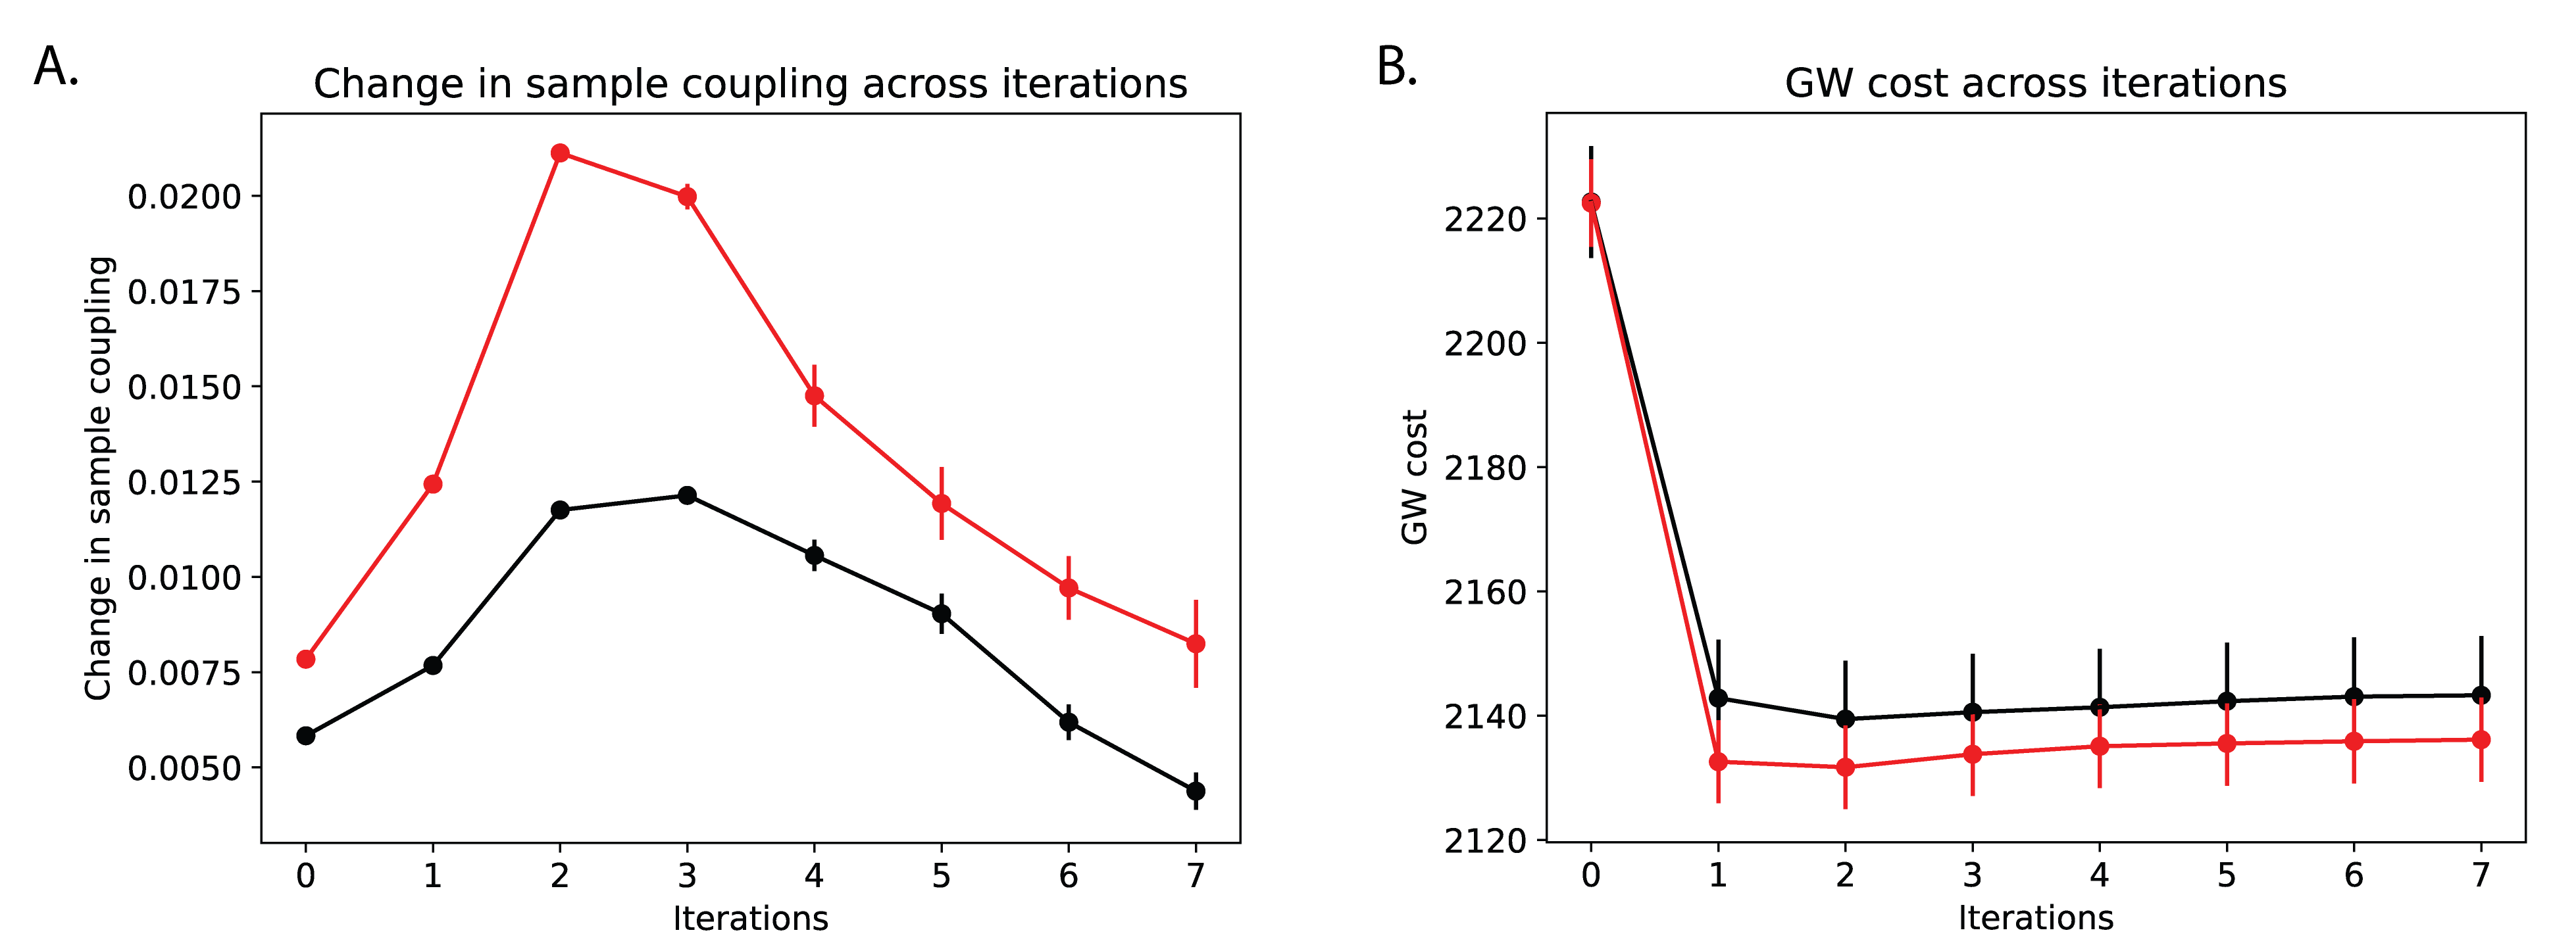
\includegraphics[width=\linewidth]{./Chapitre5/fig/timing_plots.png}
%     \caption{\label{fig:SI-timing} \textbf{(A)} Magnitude of the update made to the sample coupling
%     across iterations in AGW and GW, depicted as an example on the ``A$\rightarrow$A''
%     scenario of the HDA experiments. Error bars are based on 10 runs with random sampling.
%     We visualize the first 8 iterations as some runs converge in 8 iterations for AGW.
%     \textbf{(B)} GW distance across iterations.}
% \end{figure}